%------------------------------------------------------------------------------------
%	CHAPTER 4
%------------------------------------------------------------------------------------
\chapterimage{headConceito.png}
\chapter{Modelos Iniciais}

\begin{remark}
Na vida, não existe nada a temer, mas a entender. (Marie Curie - Cientista e Vencedora 2 vezes do Prêmio Nobel) 
\end{remark}

\section{K-Means}\index{Modelos Iniciais}
Acredito que K-Means seja o modelo mais simples para começarmos, este é um algoritmo de Aprendizado Não Supervisionado, ou seja, não necessita de atributos alvo para agir, sua função é de separar as observações em grupos de modo que possamos observar melhor os dados.

Sendo assim, nosso problema para usar esse algoritmo é exatamente achar esse \textbf{k} ideal de modo que os grupos sejam separados coerentemente. Para isso existe uma técnica interessante chamada "Técnica do Cotovelo" (Elbow Technique).
\begin{figure}[H]
	\centering
	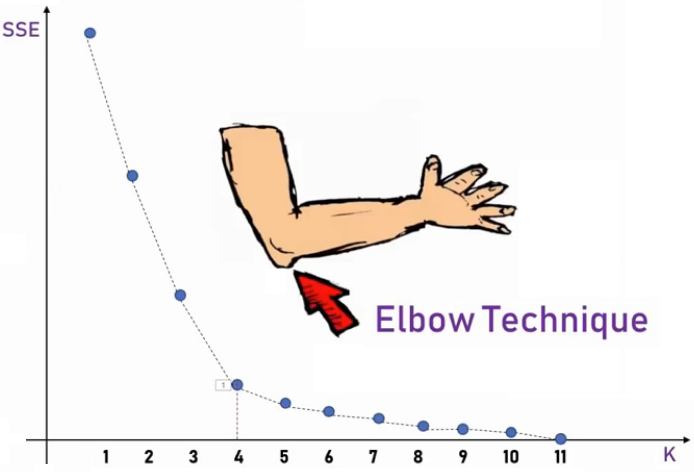
\includegraphics[width=0.46\textwidth]{cap04/tecnicaCotovelo.png}
	\caption{Técnica do Cotovelo}
\end{figure}

Exatamente na posição 4 existe uma "quebra" para passar ao próximo valor, usamos para definir essa quebra o SSE\footnote{Soma Residual dos Quadrados, é a soma dos resíduos elevado por 2. É uma medida da discrepância entre os dados e um modelo de estimativa. Um valor pequeno SSE indica um ajuste apertado do modelo aos dados.} (\textit{Sum Squared Error}).

\section{Aplicação da Técnica}\index{Modelos Iniciais}

Para achar o k ideal vamos ativar nosso JupyterLab personalizado que criamos com o Docker e na primeira célula importamos as bibliotecas necessárias:
\begin{lstlisting}[]
import pandas as pd
import numpy as np
from sklearn.preprocessing import scale
from sklearn.cluster import KMeans
from matplotlib import pyplot as plt

%matplotlib inline
\end{lstlisting}

Importamos a biblioteca Pandas e a Numpy para manipularmos os dados, a Scikit-Learn para usarmos o modelo K-Means e Matplot para vermos o resultado em um gráfico. A última linha é utilizada para mostrar os gráficos no Jupyter. Próximo passo consiste em ler os dados, baixamos o arquivo \textbf{gameML.csv} e na posição do nosso arquivo \textbf{.ipynb} criamos uma subpasta chamada \textbf{bases} e nesta colocamos o arquivo.
\begin{lstlisting}[]
df = pd.read_csv('bases/gameML.csv', delimiter=';')
df.head()
\end{lstlisting}

E como resultado da execução dessa célula devemos ter:
\begin{figure}[H]
	\centering
	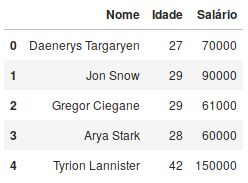
\includegraphics[width=0.4\textwidth]{cap04/baseGameML.png}
	\caption{Idades e Salários da Empresa GameML}
\end{figure}

No arquivo existem 3 campos: nome do funcionário, idade e salário, se plotarmos os dados entre idade e salário em gráfico:
\begin{lstlisting}[]
plt.scatter(df['Idade'], df['Salário'])
\end{lstlisting}

Obtemos como resultado:
\begin{figure}[H]
	\centering
	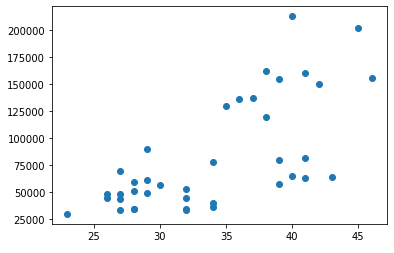
\includegraphics[width=0.55\textwidth]{cap04/plotarSalarioIdade.png}
	\caption{Idades e Salários da Empresa GameML}
\end{figure}

Quantos grupos de dados podemos distinguir? Para localizarmos a quantidade ideal aplicamos a técnica do cotovelo que consiste de:
\begin{lstlisting}[]
k_rng = range(1,10)
sse = []
for k in k_rng:
  km = KMeans(n_clusters=k)
  km.fit(df[['Idade','Salário']])
  sse.append(km.inertia_)
plt.xlabel('K')
plt.ylabel('SSE (Sum Squared Error)')
plt.plot(k_rng, sse)
\end{lstlisting}

Criar um range de 1 a 10 (um simples número máximo de possíveis \textit{clusters}), para cada valor treinamos o modelo com as variáveis e obtemos o valor do atributo \textbf{inércia}. O algoritmo agrupa dados e procura separar amostras em n grupos de igual variação, minimizando um critério conhecido como inércia ou \textbf{RSS} dentro do \textit{cluster}. O que estamos fazendo na prática e colocar o valor 1 para o \textbf{k} e guardar esse valor, em seguida o valor 2 e assim sucessivamente. Por fim plotamos esse valor em um gráfico e obtemos como resultado:
\begin{figure}[H]
	\centering
	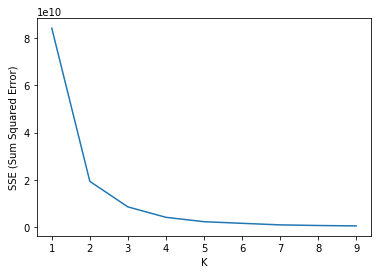
\includegraphics[width=0.53\textwidth]{cap04/aplicarCotovelo.png}
	\caption{Gráfico com os valores de Inércia}
\end{figure}

E vemos nosso "cotovelo" da curva bem na posição \textbf{3}, marcando assim o número ideal de clusters.

\section{Plotagem do Resultado do Modelo}\index{Modelos Iniciais}
Um detalhe interessante que para usarmos o algorítimo K-Means, devemos colocar os dados em "escala", vamos tentar usar o modelo sem proceder dessa forma:
\begin{lstlisting}[]
km = KMeans(n_clusters=3)
y_predict = km.fit_predict(df[['Idade','Salário']])
df['ypred'] = y_predict
df.head()
\end{lstlisting}

Já sabemos que o valor de 3 clusters é o ideal, então realizamos o treinamento com os atributos Idade e Salário para montamos um novo atributo com o resultado dessa predição (somente para que o gráfico apareça separado por cores). E plotamos o gráfico:
\begin{lstlisting}[]
cores = np.array(['green', 'red', 'blue'])
plt.scatter(x=df['Idade'],
y=df['Salário'],
c=cores[df.ypred], s=50)
\end{lstlisting}

Obtemos como resultado:
\begin{figure}[H]
	\centering
	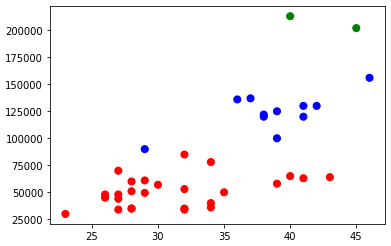
\includegraphics[width=0.55\textwidth]{cap04/separado3gruposSemEscala.png}
	\caption{Separados por Grupo}
\end{figure}

E parece que temos algo bem errado com alguns \textit{outliers} aparecendo, observamos o ponto azul no meio dos vermelhos e um outro azul isolado perto dos verdes. Então antes de treinarmos esse algoritmo devemos colocar os dados na mesma em escala, isso é feito assim:
\begin{lstlisting}[]
df['Salário'] = scale(df.Salário)
df['Idade'] = scale(df.Idade)
df.head()
\end{lstlisting}

Os atributos \textbf{idade} e \textbf{salário} possuem valores bem diferentes e distantes e isso gera problemas para nosso resultado final, colocar em escala e aproximar (sem modificar o resultado final) os valores seria algo criar um modelo de um prédio porém mantendo as mesmas proporções do prédio original.

A função da \textbf{Scikit-Learn} que realiza este processo é chamada \textit{scale()} e colocamos em escala os atributos se visualizarmos nossos dados agora veremos que o atributo \textbf{idade} possui valores entre -2 e 2 enquanto que \textit{salário} entre -1.5 e 3 (são diferentes exatamente para manter a proporcionalidade). Retornamos ao mesmo processo de treinamento:
\begin{lstlisting}[]
km = KMeans(n_clusters=3)
y_predict = km.fit_predict(df[['Idade','Salário']])
df['ypred'] = y_predict
df.head()
\end{lstlisting}

Plotamos novamente o gráfico e agora como resultado teremos:
\begin{lstlisting}[]
cores = np.array(['green', 'red', 'blue'])
plt.scatter(x=df['Idade'],
y=df['Salário'],
c=cores[df.ypred], s=50)
\end{lstlisting}

E obtemos como resultado:
\begin{figure}[H]
	\centering
	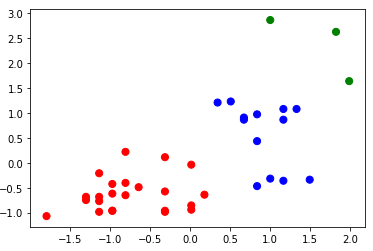
\includegraphics[width=0.55\textwidth]{cap04/separado3gruposEmEscala.png}
	\caption{Separados por Grupo em Escala}
\end{figure}

Que é um resultado bem mais coerente.

\section{K-Nearest Neighbors}\index{Modelos Iniciais}
Ou simplesmente KNN. Modelos assim existem pois muitas pessoas pensam que separar em \textit{clusters} não auxilia na predição, pois bem nosso próximo modelo é um supervisionado e destinado a Predição por Clusterização (ou se prefere por proximidade dos grupos). KNN que normalmente é usado para a predição de imagens como: Isso é um Gato? Ou não é um Gato? Porém ao invés de imagens, vamos usar uma base bem conhecida chamada \textbf{Flores Íris} para entendermos seu comportamento. 
\begin{figure}[H]
	\centering
	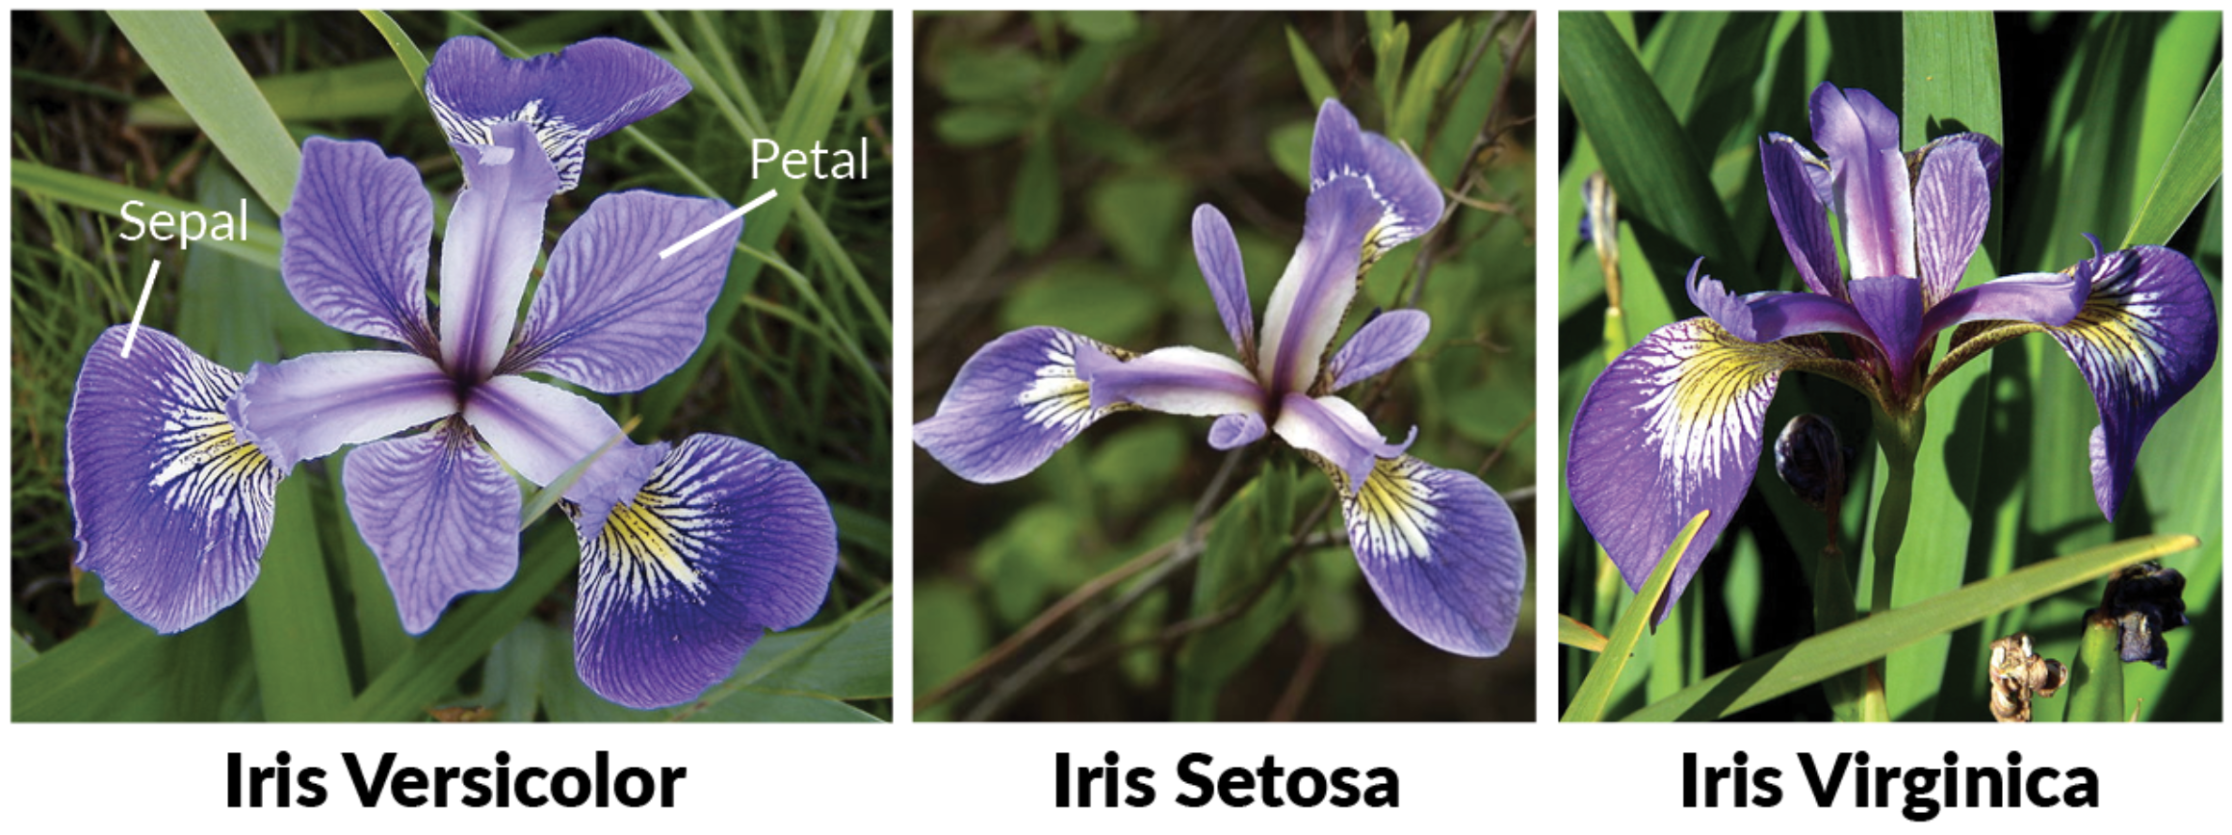
\includegraphics[width=0.65\textwidth]{cap04/iris.png}
	\caption{Flores Iris}
\end{figure}

Nessa base existem três espécies separadas: Versicolor, Setosa e Virgínica. E para distingui-las utilizamos 2 medidas da sépala e da pétala (largura e altura de cada). O problema é que algumas espécies causam as maiores confusões em nossos modelos. Para realizarmos uma predição sobre essa base importamos nossas bibliotecas:
\begin{lstlisting}[]
import numpy as np
from matplotlib import pyplot as plt
from sklearn import datasets
from sklearn.model_selection import train_test_split
from sklearn import neighbors

%matplotlib inline
\end{lstlisting}

Usamos a \textbf{NumPy} para gerenciamento dos dados. \textbf{MatPlotLib} para plotarmos os gráficos. Da \textbf{Scikit-Learn} obtemos os nossos dados através do pacote \textbf{datasets} e para separar uma massa de teste contamos com o \textit{train\_test\_split}. E a \textit{neighbors} contém o nosso algoritmo. O próximo passo consiste na preparação dos dados:
\begin{lstlisting}[]
iris = datasets.load_iris()
X, y = iris.data, iris.target

X_train, X_test, y_train, y_test = train_test_split(X, y, test_size=0.2, random_state=1234)
\end{lstlisting}

O método \textit{load\_iris()} traz a nossa base em uma matriz de dados. Nossa base está dividida em \textit{data} que contém os \textit{features} preditores (tamanho e largura da sépala e tamanho e largura da pétala, que colocaremos em X) e \textit{target}, \textit{feature} que contém a definição da espécie (0 representa \textbf{Setosa}, 1 para \textbf{Versicolor} e 2 para \textbf{Virgínica} que colocaremos em y). Usamos o método \textit{train\_test\_split} para retirar 20\% dos dados como amostra de teste e assim teremos quatro agrupamentos:
\begin{itemize}[nolistsep]
	\item \textbf{X\_train}, com os dados para treino do algorítimo.
	\item \textbf{X\_test}, com os dados para teste.
	\item \textbf{y\_train}, com o resultado para o treino.
	\item \textbf{y\_test}, com o resultado para o teste.
\end{itemize}

Com nossos dados preparados vamos treinar o modelo:
\begin{lstlisting}[]
clf = neighbors.KNeighborsClassifier()
clf.fit(X_train, y_train)
print(clf.score(X_test, y_test))
\end{lstlisting}

E conseguimos uma boa acurácia com incríveis 96\% de precisão, agora é vermos na prática como isso funciona. 

\subsection{Predição com K-Nearest Neighbors}\index{Modelos Iniciais}
Primeiro vamos mostrar os dados:
\begin{lstlisting}[]
cores = np.array(['green', 'red', 'blue'])
subplt1 = plt.scatter(x=X[:, 0], y=X[:, 1], c=cores[y], s=50)
\end{lstlisting}

Pegamos as duas primeiras variáveis tamanho e largura da sépala e obtemos como resultado:
\begin{figure}[H]
	\centering
	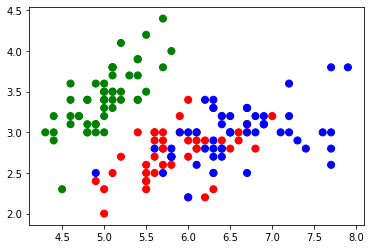
\includegraphics[width=0.5\textwidth]{cap04/knn1.png}
	\caption{Comparar tamanho e largura da Sépala}
\end{figure}

Não nos percamos nas cores \textbf{Verde} é Setosa, \textbf{Vermelho} é Versicolor e \textbf{Azul} é Virgínica. Agora vamos pensar em um ponto qualquer nesse espaço, por exemplo:
\begin{figure}[H]
	\centering
	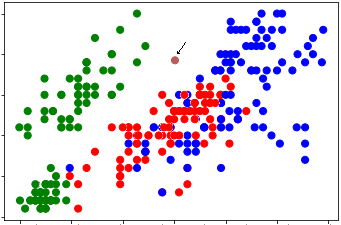
\includegraphics[width=0.5\textwidth]{cap04/acharPonto.png}
	\caption{Localizar o Ponto Roxo}
\end{figure}

O ponto roxo fica na interseção do 4º valor de X e y qual cor real ele seria? Observamos no gráfico anterior que os pontos são 6,0 e 4,0 porém nos falta o valor para mais dois atributos tamanho e largura da pétala:
\begin{lstlisting}[]
cores = np.array(['green', 'red', 'blue'])
subplt1 = plt.scatter(x=X[:, 2], y=X[:, 3], c=cores[y], s=50)
\end{lstlisting}

E obtemos como resultado:
\begin{figure}[H]
	\centering
	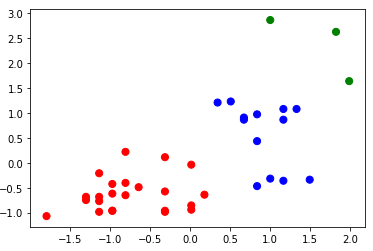
\includegraphics[width=0.55\textwidth]{cap04/separado3gruposEmEscala.png}
	\caption{Comparar tamanho e largura da Pétala}
\end{figure}

E verificamos que na interseção do 4º valor de X e y temos os valores 4,0 e 2,0. Agora que obtemos os quatro valores podemos realizar uma predição:
\begin{lstlisting}[]
predicao = clf.predict([[6.0, 4.0, 4.0, 2.0]])
print(predicao)
\end{lstlisting}

E resulta que o modelo prevê que é do tipo [1], ou seja, um ponto vermelho da espécie \textbf{Versicolor}. 

\section{Análise de Cluster}\index{Modelos Iniciais}
Então sabemos agora que ambos modelos K-Means e KNN trabalham utilizando \textit{clusters} (agrupamentos) sendo que o primeiro é do tipo não supervisionado destinado a separação com base em um número de centroides (k) presentes e os valores médios mais próximos (isso representa uma distância Euclidiana entre as observações). Porém é necessário colocar os dados em escala para verificar se não ocorre nenhuma pertubação nesse centroide. Vamos importar algumas bibliotecas para realizarmos mais testes:
\begin{lstlisting}[]
import numpy as np
import pandas as pd
import seaborn as sns
import matplotlib.pyplot as plt
from sklearn import datasets
from sklearn.preprocessing import scale
from sklearn.cluster import KMeans
from sklearn.metrics import classification_report

%matplotlib inline
\end{lstlisting}

Já passamos por todas e não desejo ser repetitivo porém dessa vez vamos utilizar a Pandas para manipular os dados e a classe \textit{metrics} da SciKit-Learn para mostrar o comportamento do nosso modelo. Iremos continuar usando a base Iris e construímos um \textit{DataFrame} somente com os dados dos atributos preditores porém guardaremos o atributo alvo para verificar como nosso modelo se comportou:
\begin{lstlisting}[]
iris = datasets.load_iris()
X = scale(iris.data)
y = pd.DataFrame(iris.target)
y.columns = ['Targets']
variable_names = iris.feature_names
iris_df = pd.DataFrame(iris.data)
iris_df.columns = variable_names
iris_df.head()
\end{lstlisting}

E nosso \textit{DataFrame} se apresenta da seguinte maneira:
\begin{figure}[H]
	\centering
	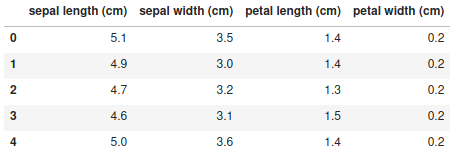
\includegraphics[width=0.4\textwidth]{cap04/dadosIris.png}
	\caption{DataFrame com os dados dos Atributos Preditores}
\end{figure}

O próximo passo é construir e treinar nosso modelo:
\begin{lstlisting}[]
clustering = KMeans(n_clusters=3, random_state=5).fit(X)
\end{lstlisting}

Normalmente para treinar um modelo passamos dois conjuntos de dados, porém o K-Means só recebe um único conjunto, exatamente por não realizar predições precisa apenas dos dados para separá-los em conjuntos. Mas como será que foi seu comportamento? Descobrimos isso comparando dois gráficos:
\begin{lstlisting}[]
cores = np.array(['green', 'red', 'blue'])
relabel = np.choose(clustering.labels_, [1, 0, 2]).astype(np.int64)
plt.figure(figsize = [15, 5])

plt.subplot(1, 4, 1)
plt.scatter(x=iris_df['petal length (cm)'], 
y=iris_df['petal width (cm)'], 
c=cores[iris.target], s=50)
plt.title('Real (Pétala)')

plt.subplot(1, 4, 2)
plt.scatter(x=iris_df['petal length (cm)'], 
y=iris_df['petal width (cm)'], 
c=cores[relabel], s=50)
plt.title('KMeans (Pétala)')

plt.subplot(1, 4, 3)
plt.scatter(x=iris_df['sepal length (cm)'], 
y=iris_df['sepal width (cm)'], 
c=cores[iris.target], s=50)
plt.title('Real (Sépala)')

plt.subplot(1, 4, 4)
plt.scatter(x=iris_df['sepal length (cm)'], 
y=iris_df['sepal width (cm)'], 
c=cores[relabel], s=50)
plt.title('KMeans (Sépala)')

plt.show()
\end{lstlisting}

Usamos os mesmos conjuntos de cores para cada espécie, teremos quatro gráficos comparativos: 1º largura e altura da Pétala e a cor será mostrada com base em nosso atributo alvo (ou seja o valor real), 2º o que o modelo achou que seria o correto, 3º largura e altura da Sépala e o 4º novamente como o modelo separou. E obtemos como resultado:
\begin{figure}[H]
	\centering
	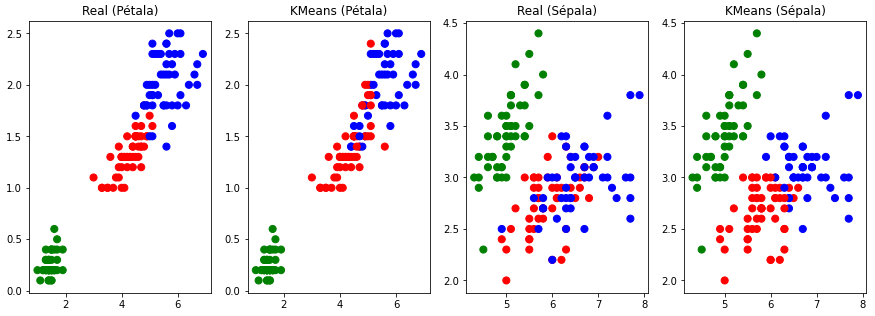
\includegraphics[width=0.8\textwidth]{cap04/comparativo.png}
	\caption{Comparativo entre o Real e o KMeans}
\end{figure}

Para pétala o \textbf{K-Means} quase acertou a posição de cada espécie, porém para Sépala aconteceram as maiores confusões, isso se deve ao fato do centroide. Para melhor avaliarmos nosso modelo precisamos de mais medidas: \textit{Precision} (precisão) é a medida de relevância do modelo, \textit{Recall} (revocação ou sensibilidade) se trata da medida de completude do modelo e \textit{F1 Score} se trata de uma média ponderada entre \textit{precision} e \textit{recall}. Podemos obtê-las da seguinte forma:
\begin{lstlisting}[]
metricas = classification_report(y, relabel)
print(metricas)
\end{lstlisting}

Obtemos como resultado:
\begin{figure}[H]
	\centering
	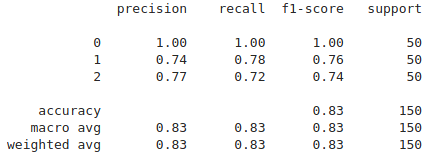
\includegraphics[width=0.6\textwidth]{cap04/relatorio.png}
	\caption{Relatório de Performance do K-Means}
\end{figure}

\textit{Precision} - É a razão entre as observações positivas previstas corretamente e o total de observações positivas previstas. Calculada com a fórmula: $TP \div (TP + FP)$.

\textit{Recall} - É a razão entre as observações positivas previstas corretamente e todas as observações da classe real. Calculada com a fórmula: $TP \div (TP + FN)$

\textit{F1 Score} - Essa pontuação leva em consideração tanto os falsos positivos quanto os negativos. Intuitivamente, não é tão fácil entender como precisão, mas F1 é geralmente mais útil que \textit{precision}, especialmente se estivermos com uma distribuição de classe desigual. $2 \times (recall \times precision) \div (recall + precision)$

\textit{Acurácia} funciona melhor se os falsos positivos e negativos tiverem um custo semelhante. Se o custo for muito diferente, é melhor olharmos essas métricas. 

\section{Clusterização Hierárquica}\index{Modelos Iniciais}
Este é um modelo alternativo ao particionamento de \textit{cluster} no conjunto de dados, pode ser aplicado para encontrar a distância entre cada ponto e seus vizinhos mais próximos e conectá-lo de forma ideal. Podemos mostrar o número de subgrupos com o auxílio de um Dendrograma\footnote{É um gráfico em formato de árvore que mostra visualmente os relacionamentos entre as observações.}. 

É útil pois não existe necessidade de especificar o número de \textit{clusters} (ou K) antes da análise e o dendrograma fornece uma representação visual desses. Vamos trazer para o conjunto de bibliotecas visto anteriormente mais três:
\begin{lstlisting}[]
from scipy.cluster.hierarchy import dendrogram, linkage
from sklearn.cluster import AgglomerativeClustering
from sklearn.metrics import accuracy_score
\end{lstlisting}

Para este exemplo vamos utilizar outra base que está contida no arquivo \textbf{mtcars.csv} (trazer essa para a subpasta \textbf{/base}). E carregamos os dados do seguinte modo:
\begin{lstlisting}[]
carros = pd.read_csv('bases/mtcars.csv')
carros.columns = ['name', 'mpg', 'cil', 'disp', 'hp', 'drat', 'wt', 'qsec', 'vs', 'am', 'gear', 'carb']
X = carros[['mpg', 'disp','hp', 'wt']].values
y = carros['am'].values
\end{lstlisting}

Essa base contém 32 modelos de carros com os seguintes atributos: Nome, autonomia em milhas por galão, número de cilindros, deslocamento (medida de poder do carro em polegada cúbica), cavalos de força, relação do eixo traseiro, peso (em libras), eficiência do gasto de combustível (por 1/4 milha), motor (0 = V-shaped, 1 = straight), câmbio (0 = automática, 1 = manual), total de marchas e carburadores. Porém para não trabalharmos com tantos atributos vamos usar somente: consumo de gasolina (mpg), deslocamento (disp), cavalos de força (hp) e peso (wt) e o nosso objetivo e descobrir se o carro possui um câmbio manual ou automático.

Podemos montar o dendrograma do seguinte modo: 
\begin{lstlisting}[]
z = linkage(X, 'ward')
dendrogram(z, truncate_mode='lastp', p=12, leaf_rotation=45, leaf_font_size=15, show_contracted=True)

plt.title('Dendograma')
plt.xlabel('Tamanho do Cluster')
plt.ylabel('Distancia')
plt.axhline(y=500)
plt.axhline(y=150)
plt.show()
\end{lstlisting}

Obtemos como resultado:
\begin{figure}[H]
	\centering
	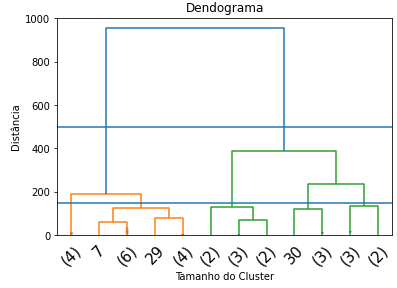
\includegraphics[width=0.6\textwidth]{cap04/dendrograma.png}
	\caption{Dendrograma dos tamanhos do Cluster}
\end{figure}

O dendrograma mostra como cada \textit{cluster} é composto e desenha um link em forma de U entre cada cluster e seus filhos. A parte superior indica uma mesclagem. Cada perna indica quais foram mesclados. O comprimento das pernas e do U representa a distância entre os filhos.

Para mesclar recursivamente o par de \textit{clusters} e aumentar minimamente a distância de ligação utilizamos a função AgglomerativeClustering(). Essa possui dois parâmetros básicos: \textit{affinity} e \textit{linkage}.

\textit{affinity}: métrica utilizada para calcular a ligação. Possui as seguintes opções:
\begin{itemize}[nolistsep]
	\item \textit{euclidean} - é o único que aceita o parâmetro \textit{linkage} como \textit{ward}. Refere-se a distância euclidiana que pode ser provada pela aplicação repetida do teorema de Pitágoras.
	\item \textit{l1} - critério de erro absoluto.
	\item \textit{l2} - critério de erros quadrados (lembramos do RSS).
	\item \textit{manhattan} - distância euclidiana ao quadrado.
	\item \textit{cosine} - também chamada de Similaridade do Cosseno. É a distância do cosseno entre duas variáveis.
	\item \textit{precomputed} - necessita de uma matriz de distância (em vez de similaridade) como entrada para o método de ajuste, pois X será considerado uma matriz.
\end{itemize}

\textit{linkage}: define qual o critério de ligação usar. Determina qual distância usar entre os conjuntos de observação. Possui as seguintes opções:
\begin{itemize}[nolistsep]
	\item \textit{ward} - minimiza a variação dos \textit{clusters} que estão sendo mesclados.
	\item \textit{average} - média das distâncias de cada observação dos conjuntos.
	\item \textit{complete} - distâncias máximas entre todas as observações dos dois conjuntos.
	\item \textit{single} - mínimo das distâncias entre todas as observações dos dois conjuntos.
\end{itemize}

Como escolher os parâmetros ideais? Fácil, testemos várias combinações e veremos qual possui uma melhor acurácia para os dados que estamos tratando:
\begin{lstlisting}[]
hclusters1 = AgglomerativeClustering(n_clusters=2, affinity='euclidean', linkage='ward').fit(X)
print('Método 1:', accuracy_score(y, hclusters1.labels_))

hclusters2 = AgglomerativeClustering(n_clusters=2, affinity='euclidean', linkage='complete').fit(X)
print('Método 2:', accuracy_score(y, hclusters2.labels_))

hclusters3 = AgglomerativeClustering(n_clusters=2, affinity='euclidean', linkage='average').fit(X)
print('Método 3:', accuracy_score(y, hclusters3.labels_))

hclusters4 = AgglomerativeClustering(n_clusters=2, affinity='manhattan', linkage='single').fit(X)
print('Método 4:', accuracy_score(y, hclusters4.labels_))

hclusters5 = AgglomerativeClustering(n_clusters=2, affinity='manhattan', linkage='complete').fit(X)
print('Método 5:', accuracy_score(y, hclusters5.labels_))

hclusters6 = AgglomerativeClustering(n_clusters=2, affinity='manhattan', linkage='average').fit(X)
print('Método 6:', accuracy_score(y, hclusters6.labels_))

hclusters7 = AgglomerativeClustering(n_clusters=2, affinity='cosine', linkage='single').fit(X)
print('Método 7:', accuracy_score(y, hclusters7.labels_))

hclusters8 = AgglomerativeClustering(n_clusters=2, affinity='cosine', linkage='complete').fit(X)
print('Método 8:', accuracy_score(y, hclusters8.labels_))

hclusters9 = AgglomerativeClustering(n_clusters=2, affinity='cosine', linkage='average').fit(X)
print('Método 9:', accuracy_score(y, hclusters9.labels_))
\end{lstlisting}

Obtemos como resultado: \\
{\ttfamily Método 1: 0.78125 \\
Método 2: 0.4375 \\
Método 3: 0.78125 \\
Método 4: 0.625 \\
Método 5: 0.71875 \\
Método 6: 0.71875 \\
Método 7: 0.3125 \\
Método 8: 0.28125 \\
Método 9: 0.1875}

Assim para esse caso \textit{Euclidian/Ward} ou \textit{Manhattan/Complete} são os que melhor responderam ao nosso conjunto de dados com uma acurácia de 78,12\%. Podemos inclusive tirar um relatório mais completo (como já vimos):
\begin{lstlisting}[]
print(classification_report(y, hclusters1.labels_))
\end{lstlisting}

Obtemos como resultado:
\begin{figure}[H]
	\centering
	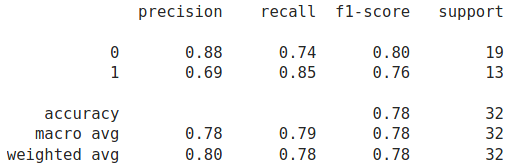
\includegraphics[width=0.6\textwidth]{cap04/relatorioHie.png}
	\caption{Relatório de Performance da Clusterização Hierárquica}
\end{figure}


Só que ficou uma pergunta no ar, esse método se comporta melhor que um modelo de clusterização preditivo como o KNN?

\subsection{Clusterização Hierárquica versus K-Nearest Neighbors}\index{Modelos Iniciais}
Para verificar como o KNN se comporta com os dados dos carros adicionamos mais quatro bibliotecas:
\begin{lstlisting}[]
from sklearn.neighbors import KNeighborsClassifier
from sklearn import preprocessing
from sklearn.model_selection import train_test_split
from sklearn.metrics import classification_report
\end{lstlisting}

Como já temos nossos dados, vamos apenas separá-los em bases de treino e teste:
\begin{lstlisting}[]
X = preprocessing.scale(X)
X_treino, X_teste, y_treino, y_teste = train_test_split(X, y, test_size=.20, random_state=17)
\end{lstlisting}

Porém devemos sempre lembrar que os modelos de clusterização trabalham melhor quando os dados estão em escala, assim acertamos os atributos preditores antes de realizar a separação de 80\% dos dados para treino e 20\% para teste.
\begin{lstlisting}[]
clf = KNeighborsClassifier()
clf.fit(X_treino, y_treino)
\end{lstlisting}

Treinamos nosso modelo e podemos avaliar o resultado:
\begin{lstlisting}[]
y_predito = clf.predict(X_teste)
print(classification_report(y_teste, y_predito))
\end{lstlisting}
	
Obtemos como resultado:
\begin{figure}[H]
	\centering
	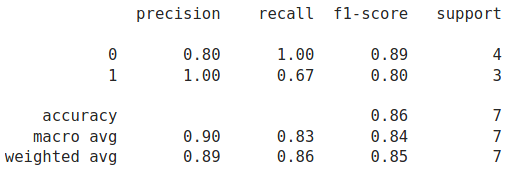
\includegraphics[width=0.5\textwidth]{cap04/relatorioKNN.png}
	\caption{Relatório de Performance do K-Nearest Neighbors}
\end{figure}

E na média percebemos que este se comporta melhor pois atinge resultados acima dos 80\%.

\section{Regressão Linear}\index{Modelos Iniciais}
A regressão linear tenta modelar o relacionamento entre dois atributos, através de ajustes sob uma equação linear dos dados observados. Um atributo é considerado \textbf{explicativo} e a outro \textbf{dependente}. Para simplificar um pouco, é uma técnica que utiliza valores de entrada para predizer os de saída (como por exemplo, prever o crescimento da população de um País) através da aplicação dos coeficientes (também chamados de peso) da equação linear. 

Comecemos com a importação das bibliotecas que necessitamos:
\begin{lstlisting}[]
import pandas as pd
import numpy as np
from matplotlib import pyplot as plt
from sklearn.linear_model import LinearRegression

%matplotlib inline
\end{lstlisting}

A classe \textit{Linear Model} da \textit{Scikit-Learn} o método \textit{LinearRegression} para realizar nosso trabalho. Baixar a base de dados \textbf{PopBrasil.csv} que contém as observações de Crescimento da População Brasileira.
\begin{lstlisting}[]
df = pd.read_csv('bases/PopBrasil.csv')
df.head()
\end{lstlisting}

Obtemos como resultado:
\begin{figure}[H]
	\centering
	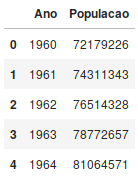
\includegraphics[width=0.15\textwidth]{cap04/basePop.png}
	\caption{Dados da População Brasileira}
\end{figure}

Devemos saber que o modelo trabalha com a relação entre atributos numéricos: explanatórios X e dependentes y. Utiliza somente esse tipo devido aos ajustes matemáticos que são realizados e os pesos criados conforme a função minimiza os erros. Nossas observações são bem simples: temos atributos numéricos, "Ano" e "População". Para entendermos o relacionamento entre os atributos, plotamos esses em um gráfico:
\begin{lstlisting}[]
plt.xlabel('Ano')
plt.ylabel('Quantidade da População')
plt.scatter(df.Ano, df.Populacao, color='red', marker='+')
\end{lstlisting}

Obtemos como resultado:
\begin{figure}[H]
	\centering
	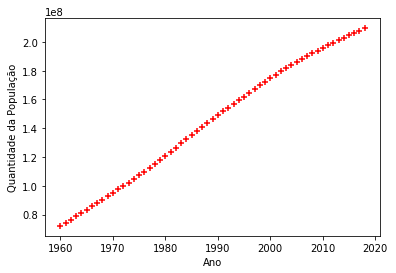
\includegraphics[width=0.4\textwidth]{cap04/grafRelAnoPop.png}
	\caption{Dados da População Brasileira}
\end{figure}

E esta é a parte mais importante na execução desse modelo, a medida que alteramos o valor de "Ano" o valor de "População" também é afetado, ou seja, existe um relacionamento linear. Essa é a premissa básica para se usar este algoritmo, o relacionamento forte entre os atributos deve existir.

\subsection{Aplicar a Regressão Linear}\index{Modelos Iniciais}

Agora que temos nossos atributos conferidos, basta treinarmos nosso modelo e obtermos nossa previsão:
\begin{lstlisting}[]
reg = LinearRegression()
reg.fit(df[['Ano']], df.Populacao)
prev = reg.predict([[2020]])
print("Previsão 2020 é: %d" % prev)
\end{lstlisting}

E teremos a predição da população brasileira para o ano de 2020, que é 221.322.254 de habitantes. Como a magia acontece? Pura matemática que é fornecida pela seguinte fórmula:
\begin{figure}[H]
	\centering
	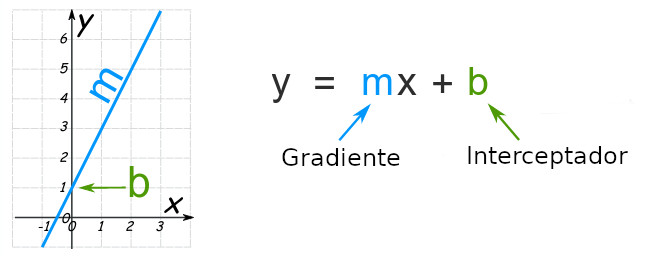
\includegraphics[width=0.5\textwidth]{cap04/formulaRL.png}
	\caption{Base da Regressão Linear}
\end{figure}

\begin{note}[Para saber mais]{}
	Se deseja conhecer mais sobre o assunto, visite a página: \url{https://www.mathsisfun.com/algebra/linear-equations.html} aonde se obtém uma explicação mais completa.
\end{note}

E podemos reproduzir esse resultado pois o objeto treinado nos fornece tanto o valor do Gradiente (\textit{coef\_[0]}) quanto do Interceptador (\textit{intercept\_}). Então:
\begin{lstlisting}[]
m = reg.coef_[0]
b = reg.intercept_
prev2020 = m * 2020 + b
print("Previsão 2020 é: %d" % prev2020)
\end{lstlisting}

E temos exatamente o mesmo resultado. Podemos traçar a "Reta da Regressão Linear", pois o modelo consegue predizer os resultados de cada ano:
\begin{lstlisting}[]
plt.xlabel('Ano')
plt.ylabel('Quantidade da População')
plt.scatter(df.Ano, df.Populacao, color='red', marker='+')
plt.plot(df.Ano, reg.predict(df[['Ano']]), color='blue')
\end{lstlisting}

Obtemos como resultado:
\begin{figure}[H]
	\centering
	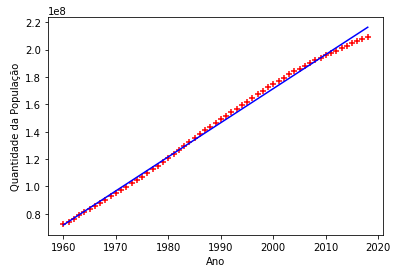
\includegraphics[width=0.5\textwidth]{cap04/grafRelAnoPopReta.png}
	\caption{Dados da População Brasileira com a Previsão}
\end{figure}

Vamos praticar nossos novos "poderes de futurólogo", junto a essa base encontramos outra chamada ExpecVida.csv, com ela, tente prever qual será a Expectativa de Vida do brasileiro no ano de 2020.

\subsection{Regressão Linear com mais de um Preditor}\index{Modelos Iniciais}
Vimos como usar o modelo de Regressão Linear, porém apenas a título de facilitação do entendimento, somente um atributo preditor. Mas o que acontece quando o alvo é influenciado por mais de um preditor? Vamos entender na prática como isso acontece.

Pensemos em um caso do Varejo, vamos utilizar um conjunto de observações chamado \textbf{marketSales.csv} que como o nome sugere, são compostos por transações de vendas. Sabemos que várias coisas influenciam a saída de um determinado produto, tais como, o grau de visibilidade, peso, se possui muita ou pouca quantidade de gordura, tamanho do mercado ou outros.

Começamos com a importação da bibliotecas necessárias:
\begin{lstlisting}[]
import pandas as pd
from sklearn.linear_model import LinearRegression
from sklearn.preprocessing import LabelEncoder
from sklearn.model_selection import train_test_split
from matplotlib import pyplot as plt

%matplotlib inline
\end{lstlisting}

E ler nossa base de dados:
\begin{lstlisting}[]
df = pd.read_csv('bases/marketSales.csv')
df.head()
\end{lstlisting}

Até o momento nada de novo, nosso problema começa ao repararmos nas observações:
\begin{figure}[H]
	\centering
	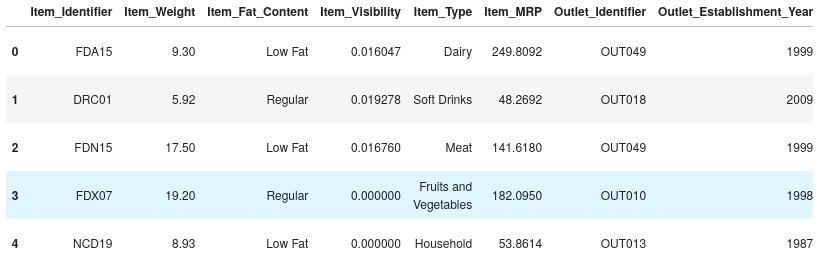
\includegraphics[width=0.5\textwidth]{cap04/dadosMarket.png}
	\caption{Observações sobre Vendas de Produtos}
\end{figure}

Sabemos que os modelos de regressão só trabalham com tipos numéricos, muito pior existe o caso de nulos entre algumas outras inconsistências  nessas 14.204 observações.

\subsection{Regressão Linear e Limpeza dos Dados}\index{Modelos Iniciais}

Sejamos francos, maior parte de trabalho do Cientista de Dados é arrumar os dados que sofridamente conseguiu para realizar o trabalho, então começaremos a compreender como uma parte disso funciona. Primeiro detalhe vamos tratar os atributos indesejáveis, nulos e que não contribuem em absolutamente em nada para o aumento/diminuição das vendas. Atributos como o código identificador do produto (\textit{Item\_Identifier}) e  código identificador do mercado (\textit{Outlet\_Identifier}) - por esse motivo que o Cientista de Dados deve entender do negócio.

Ao verificarmos a função \textit{info()} descobrimos ainda que o atributo alvo (\textit{Item\_Outlet\_Sales}) que indica a quantidade de produtos vendidos possui dados nulos (ou seja, também não servem para previsão).
\begin{lstlisting}[]
df = df.drop(df[df['Item_Outlet_Sales'].isnull()].index)
df = df.drop(columns=['Item_Identifier', 'Outlet_Identifier'], axis=1)
\end{lstlisting}

Cuidado pois se aplicamos um corte seco como: {\ttfamily df.dropna(how='any',inplace=True)} teremos somente 4.650 observações (devido a eliminação dos valores nulos contidos em outros atributos) - ou seja perdemos quase 10.000 observações. Lembrar que o tratamento dos nulos deve ser cirúrgico e criterioso. Ao aplicar o corte corretamente somente do atributo alvo ficamos com 8.523 observações. Além disso removemos os preditores que não serviam.

Nosso próximo problema com nulos é nos atributos: peso do item (\textit{Item\_Weight}) e tamanho da loja (\textit{Outlet\_Size}). Em um caso de dados real devemos procurar preencher esses valores solicitando a informação necessária aos responsáveis, porém para fins desse trabalho iremos remover essa colunas também.
\begin{lstlisting}[]
df = df.drop(columns=['Item_Weight', 'Outlet_Size'], axis=1)
\end{lstlisting}

Não temos mais a presença de nulos, mas ainda temos problemas, precisamos verificar os atributos não numéricos das observações, isto é: conteúdo de gordura (\textit{Item\_Fat\_Content}), tipo do item (\textit{Item\_Type}), localização da loja (\textit{Outlet\_Location\_Type}) e tipo da loja (\textit{Outlet\_Type}). Para isso:
\begin{lstlisting}[]
print("Gordura:", df['Item_Fat_Content'].unique())
print("Tipo:", df['Item_Type'].unique())
print("Loc. Loja:", df['Outlet_Location_Type'].unique())
print("Tipo Loja:", df['Outlet_Type'].unique())
\end{lstlisting}

O atributo \textit{Item\_Fat\_Content} possui uma faixa com os seguintes valores: '\textit{LF}', '\textit{Low Fat}', '\textit{Regular}', '\textit{low fat}' ou '\textit{reg}'. Obviamente só existem dois tipos: '\textit{Low Fat}' e '\textit{Regular}' os outros três são variações desses valores. Para corrigir isso e realizar sua conversão: 
\begin{lstlisting}[]
df['Item_Fat_Content'] = df['Item_Fat_Content'].map({'LF': 1, 'Low Fat': 1, 'low fat': 1, 'reg': 2, 'Regular': 2})
df['Item_Fat_Content'] = df['Item_Fat_Content'].astype(pd.Int64Dtype())
df['Outlet_Location_Type'] = df['Outlet_Location_Type'].map({'Tier 1': 1, 'Tier 2': 2, 'Tier 3': 3})
df['Outlet_Location_Type'] = df['Outlet_Location_Type'].astype(pd.Int64Dtype())
df['Outlet_Type'] = df['Outlet_Type'].map({'Supermarket Type1': 1, 'Supermarket Type2': 2, 'Supermarket Type3': 3, 'Grocery Store': 4})
df['Outlet_Type'] = df['Outlet_Type'].astype(pd.Int64Dtype())
\end{lstlisting}

Criamos um dicionário com as faixas, repetimos os mesmos valores para os tipos que são semelhantes e realizamos a troca dos elementos no \textit{DataFrame}. Aplicamos também a mesma prática para a localização e tipo da loja que possui poucos valores. Porém ainda temos o caso de tipo do item que vamos trocá-lo de uma forma diferente (é ideal quando existem muitos valores diferentes).

Cada atributo tem um tipo determinado, por exemplo, \textit{float} aceita números com pontos decimais, \textit{int} numéricos inteiros, \textit{string} caracteres, além disso \textit{Python} trabalha com um tipo especial denominado \textit{category}. Corresponde a uma determinada faixa de valores. Converter tipo do item em atributo categórico:
\begin{lstlisting}[]
df['Item_Type'] = df.Item_Type.astype('category')
\end{lstlisting}

Uma vez realizado esse processo podemos "codificá-lo":
\begin{lstlisting}[]
le_Item_Type = LabelEncoder()
df['Item_Type'] = le_Item_Type.fit_transform(df['Item_Type'])
df.head()
\end{lstlisting}

Para cada valor categorizado é atribuído um valor numérico (ou seja o mesmo trabalho que tivemos para o mapa). Usamos as funções \textit{info()} e \textit{describe()} e podemos partir para a próxima etapa sem quaisquer problemas com os dados, pois agora são todos numéricos e não possuem qualquer valor nulo.

\subsection{Separação e treino}\index{Modelos Iniciais}

Separar em treino e teste (para avaliarmos nosso modelo) e remover o atributo alvo:
\begin{lstlisting}[]
target = df['Item_Outlet_Sales']
df = df.drop(columns=['Item_Outlet_Sales'], axis=1)
X_train, X_test, y_train, y_test = train_test_split(df, target, test_size = .2)
print('Amostra de Treino:', X_train.shape)
print('Amostra de Teste:', X_test.shape)
\end{lstlisting}

Usamos um valor de 20\% para nosso teste e temos: 6.818 observações para treino e 1.705 de teste. Treinamos nosso modelo e verificamos seu resultado:
\begin{lstlisting}[]
clf = LinearRegression()
clf.fit(X_train, y_train)
print('Acurácia: ', clf.score(X_test, y_test))
\end{lstlisting}

E obtemos uma acurácia aproximada de 42\% e qual o motivo dessa discrepância tão grande? Simples, estamos cada vez mais perto da realidade e podemos verificar que realizar previsões com altos scores e poucas ações não existe. Pois se fosse assim: Corramos para treinar um modelo que nos dará os seis números da MegaSena. Ou ao menos nos dizer quando vai chover corretamente com muito pouco trabalho. Por fim podemos ver como os dados estão bem discrepantes em relação ao que foi predito e o real:
\begin{lstlisting}[]
y_pred = model.predict(X_test)
plt.plot(y_test, y_test)
plt.scatter(y_test, y_pred, c = 'red', marker='+')
plt.ylabel('Real')
plt.xlabel('Predito')
plt.show()
\end{lstlisting}

Obtemos como resultado:
\begin{figure}[H]
	\centering
	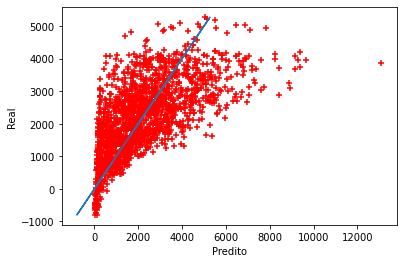
\includegraphics[width=0.5\textwidth]{cap04/regressaoFinal.png}
	\caption{Regressão Linear aplicada a vários atributos}
\end{figure}

Em vermelho são a relação entre o valor real e o que foi predito, a linha azul mostra a Reta da Regressão. Verificamos que temos um ponto bem isolado? Pode ser um \textit{outlier}? Exatamente por esse motivo que passamos um bom tempo em EDA.

\clearpage
